\documentclass{beamer}
\usepackage[utf8]{inputenc}
\usepackage{listings}
\usepackage{multicol}
\usepackage{graphicx}
\usepackage{caption}
\usepackage{soul}

\usetheme{Frankfurt}
\usecolortheme{default}


\title[Crisis]{Introduction to contract programming}
\author{Łukasz Ziobroń}
\institute{Nokia}
\date{Code Dive Community, 2015}
\subject{Computer Science}
\lstset
{
    language=C++,
    numbers=left,
    basicstyle=\ttfamily\scriptsize,
    keywordstyle=\color{blue}\ttfamily,
    stringstyle=\color{red}\ttfamily,
    commentstyle=\color{green}\ttfamily
}
\graphicspath{ {./img/} }
\DeclareGraphicsExtensions{.pdf,.png,.jpg}
\DeclareCaptionFormat{listing}{\vskip1pt#1#2#3}
\captionsetup[lstlisting]{format=listing,singlelinecheck=false}



\begin{document}


\begin{frame}
\titlepage
\end{frame}

\begin{frame}
\frametitle{Agenda}
\tableofcontents[hideallsubsections]
\end{frame}


\section{Problematic examples}
\begin{frame}
\sectionpage
\end{frame}

\subsection{Ariane 5 mission}
\begin{frame}
\frametitle{Ariane 5 mission}
\only<1>
{
  In 1996, the Ariane 5 rocket was reusing software from the Ariane 4. 37 seconds after its maiden launch the self-destruct safety mechanism was activated. \\~\\
  A data conversion from 64-bit floating point value to 16-bit signed integer value to be stored in a variable representing horizontal bias caused a processor trap because the floating point value was too large to be represented by a 16-bit signed integer. \footnote{https://en.wikipedia.org/wiki/Ariane\_5\#Notable\_launches} \\~\\
  This bug, existing in Ariane 4 software never came out on Ariane 4 rocket.
}
\only<2>{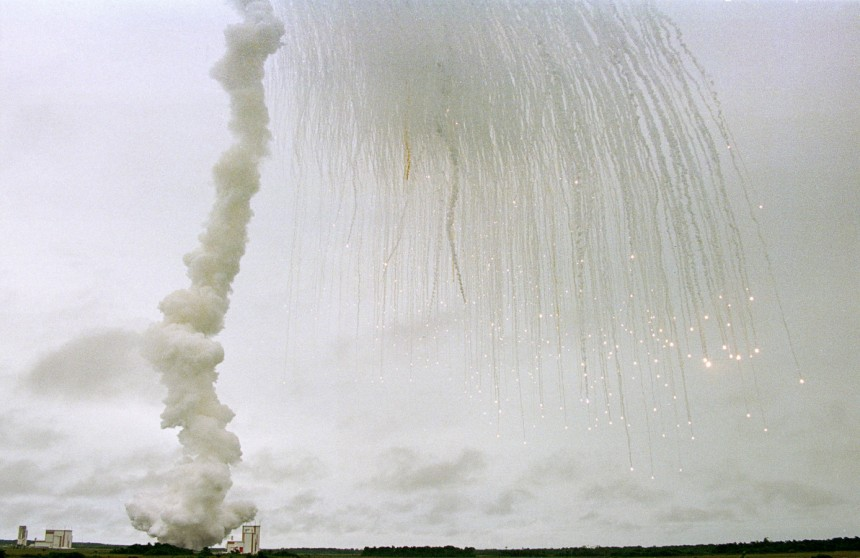
\includegraphics[scale=0.35]{ariane}}
\end{frame}

\subsection{Calculator source code}
\begin{frame}[fragile]
\frametitle{Basic calculator}
\only<1>{ \lstinputlisting[linerange={27-37}]{"src/calculator.cpp"} }
\only<2>{ \lstinputlisting[linerange={39-61}]{"src/calculator.cpp"} }
\only<3>{ \lstinputlisting[linerange={63-75}]{"src/calculator.cpp"} }
\only<4>{ \lstinputlisting[linerange={77-88}]{"src/calculator.cpp"} }
\end{frame}

\subsection{Calculator source code}
\begin{frame}[fragile]
\frametitle{Basic calculator - summary}
What should we do when input is not valid?
\pause
\begin{itemize}[<+->]
  \item nothing (very clean code, but not recommended)
  \item signal the problem (return optional, special or magic values - NaN, 0, none)
  \item throw an exception (and force the user to catch it)
  \item terminate the application that is about to enter an UB
\end{itemize}
\pause
\begin{block}{}
Proper behavior will be considered later
\end{block}
\end{frame}

\subsection{Blender interface}
\begin{frame}
\frametitle{Blender interface}

\begin{columns}
\column{.6\textwidth}
Acceptance Criteria
\begin{itemize}
  \item blender cannot run empty
  \item speed can be changed only by 1
  \item speed range is from 0 to 9 
\end{itemize}
\pause
\begin{block}{}
ATDD - Acceptance Test Driven Development
\end{block}
\column{.4\textwidth}
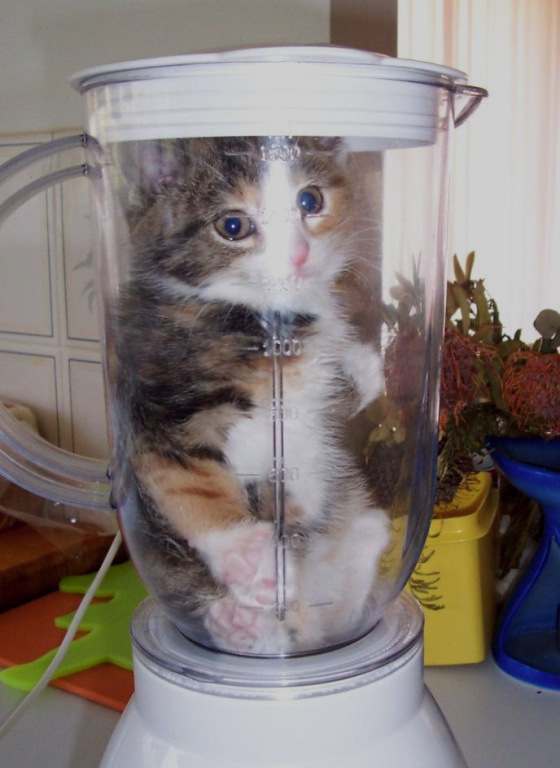
\includegraphics[scale=0.2]{kitten_in_blender}
\end{columns}
\end{frame}

\begin{frame}[fragile]
\frametitle{Blender interface}
\lstinputlisting[linerange={3-30},basicstyle=\tiny]{"src/Blender.java"}
\end{frame}


\subsection{DB query example by A. Krzemieński}
\begin{frame}[fragile]
\frametitle{DB query example by A. Krzemieński}
\lstinputlisting[linerange={-12}]{"src/db.cpp"}
\end{frame}

\begin{frame}
\frametitle{Possible inputs}
\begin{block}{When end-user is nice...}
Tom
\end{block}

\pause
\begin{block}{When end-user is malicious...}
JOHN'; delete from USERS where 'a' = 'a
\end{block}

\pause
\begin{alertblock}{Achtung!}
SQL Injection vulnerability! \\~\\
select count(*) from USERS where NAME = '\hl{JOHN'; delete from USERS where 'a' = 'a}';
\end{alertblock}
\end{frame}

\begin{frame}
\frametitle{Who is guilty?}
\lstinputlisting[linerange={-12}]{"src/db.cpp"}
\begin{block}{}
\small{Assuming that functions \textit{checkIfUserExists} and \textit{authenticate} were written by two different people, which of them is responsible for the bug?}
\end{block}
\pause
\begin{block}{}
\small{Without clearly stated expectations, it is impossible to tell whose fault it is: it is a failure to communicate between two programmers (or even one).}
\end{block}
\end{frame}

\begin{frame}
\frametitle{Let's fix it!}
We have two problems then:
\begin{itemize}
  \item the program has a bug
  \item it is not clear whose responsibility it is
\end{itemize}
\pause
\begin{block}{Implementation of name validation}
\lstinputlisting[linerange={14-19},numbers=none]{"src/db.cpp"}
\end{block}
\end{frame}

\begin{frame}
\frametitle{Let's fix it!}
\lstinputlisting[linerange={21-37}]{"src/db.cpp"}
\pause
\begin{block}{}
Nobody trusts nobody and everyone just checks for the dangerous conditions.
\end{block}
\end{frame}

\begin{frame}
\frametitle{Fixed!}
\begin{center}
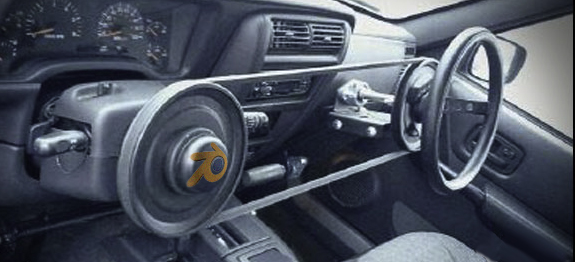
\includegraphics[scale=0.55]{steering_wheel}
\end{center}
\end{frame}

\begin{frame}
\frametitle{Problem fixed, but anothers arised}
Problems:
\begin{itemize}[<+->]
  \item Performance: checking the same condition many times
  \item Readability: code becomes messy
  \item Flow: if SIGNAL() throws someone needs to catch the exception
\end{itemize}
\pause
\begin{block}{What should SIGNAL() do?}
\pause
Whatever we choose, the program will grow in complexity; and complexity (especially a messy one like this) is likely to cause bugs.
\end{block}
\end{frame}



\section{DbC Theory}
\begin{frame}
\sectionpage
\end{frame}

\subsection{What is a contract?}
\begin{frame}
\frametitle{What is Design by Contract?}
\setbeamercovered{transparent}
\uncover<1-2>{A paradigm which was first introduced by Bertrand Meyer, the creator of Eiffel. Although Eiffel has support for programming by contract built into the language, most of the concepts can be used in any language \footnote{http://www.cs.unc.edu/~stotts/COMP204/contract.html}.  \\~\\}
\uncover<2-2>{Basically programming by contract creates a contract between the software developer and software user - in Meyer's terms the supplier and the consumer.  \\~\\}
\end{frame}

\subsection{3 assumptions}
\begin{frame}
\frametitle{3 assumptions}
\setbeamercovered{transparent}
\uncover<1-3>{Every feature, or method, starts with a \textbf{precondition} that must be satisfied by the consumer of the routine. \\~\\}
\uncover<2-3>{And each feature ends with \textbf{postconditions} which the supplier guarantees to be true (if and only if the preconditions were met). \\~\\}
\uncover<3-3>{Also, each class has an \textbf{invariant} which must be satisfied after any changes to the object represented by the class. In the other words, the invariant guarantees the object is in a valid state.}
\end{frame}

\subsection{Precondition example}
\begin{frame}[fragile]
\frametitle{Precondition example}
\lstinputlisting[linerange={17-25}]{"src/proposal.cpp"}
\end{frame}

\subsection{Postcondition example}
\begin{frame}[fragile]
\frametitle{Postcondition example}
\lstinputlisting[linerange={27-37}]{"src/proposal.cpp"}
\end{frame}

\subsection{Class invariant example}
\begin{frame}[fragile]
\frametitle{Class invariant example}
\lstinputlisting[linerange={39-50}]{"src/proposal.cpp"}
\end{frame}

\subsection{Example from latest C++ DbC proposal}
\begin{frame}
\frametitle{Example from latest C++ DbC proposal}
\lstinputlisting[linerange={1-15}]{"src/proposal.cpp"}
\pause
\begin{block}{}
Examples from C++ Design by Contract proposal: n1962, n1613.
\end{block}
\end{frame}



\section{Language support}
\begin{frame}
\sectionpage
\end{frame}

\subsection{DbC support in some languages}
\begin{frame}
\frametitle{DbC support in some languages}
\begin{itemize}
  \item C++
  \begin{itemize}
    \item GNU Nana: https://savannah.gnu.org/projects/nana
    \item Escher C++ Verifier: http://eschertech.com/products/ecv.php
    \item Loki Contract Checker: http://loki-lib.sourceforge.net
    \item Contract++: http://sourceforge.net/p/contractpp/wiki/Home
  \end{itemize}
  \item Java
  \begin{itemize}
    \item \textbf{iContract}/jContracts: http://sourceforge.net/projects/jcontracts
    \item valid4j: https://github.com/helsing/valid4j
    \item jContractor: http://jcontractor.sourceforge.net
  \end{itemize}
  \item Python
  \begin{itemize}
    \item PyContracts: https://pypi.python.org/pypi/PyContracts
    \item PyDBC: https://pypi.python.org/pypi/PyDBC
  \end{itemize}
  \item .Net
  \begin{itemize}
    \item Code Contracts: http://research.microsoft.com/en-us/projects/contracts
  \end{itemize}
  \item \textbf{D}: built-in mechanism
  \item \textbf{Eiffel}: built-in mechanism
\end{itemize}
\end{frame}

\subsection{Eiffel - it started here}
\begin{frame}[fragile]
\frametitle{Eiffel - it started here}
\lstinputlisting[linerange={1-11},language=Eiffel]{"src/examples.eiffel"}
\end{frame}

\begin{frame}[fragile]
\frametitle{Eiffel - it started here}
\lstinputlisting[linerange={13-17},language=Eiffel]{"src/examples.eiffel"}
\end{frame}

\subsection{D - built-in mechanism}
\begin{frame}[fragile]
\frametitle{D - built-in mechanism}
\lstinputlisting[linerange={1-13}]{"src/examples.d"}
\end{frame}

\begin{frame}[fragile]
\frametitle{D - built-in mechanism}
\lstinputlisting[linerange={15-24}]{"src/examples.d"}
\end{frame}

\subsection{Java - iContract}
\begin{frame}[fragile]
\frametitle{iContract - quick overview}
\lstinputlisting[linerange={1-19},language=Java]{"src/iContract.java"}
\end{frame}

\begin{frame}[fragile]
\frametitle{Java - iContract: class invariants}
\lstinputlisting[linerange={21-29},language=Java]{"src/iContract.java"}
\end{frame}

\begin{frame}[fragile]
\frametitle{Java - iContract: forall \& exists quantifiers}
\lstinputlisting[linerange={31-34},language=Java]{"src/iContract.java"}
\lstinputlisting[linerange={36-38},language=Java]{"src/iContract.java"}
\end{frame}

\begin{frame}[fragile]
\frametitle{Java - iContract: implications and logical operators}
\lstinputlisting[linerange={40-43},language=Java]{"src/iContract.java"}
\lstinputlisting[linerange={45-50},language=Java]{"src/iContract.java"}
\end{frame}

\begin{frame}[fragile]
\frametitle{Java - iContract: Stack interface example}
\begin{columns}
\column{.75\textwidth}
\lstinputlisting[linerange={3-24},language=Java]{"src/Stack.java"}
\column{.25\textwidth}
\uncover<2->{Hey man, aren't they a unit tests? \\~\\}
\uncover<3->{Maybe I can skip them? \\~\\}
\uncover<4->{You can, but don't forget to test your contracts.}
\end{columns}
\end{frame}

\begin{frame}[fragile]
\frametitle{Java - iContract: Stack interface example}
\begin{center}

\includegraphics[scale=0.6]{morpheus_ut}
\end{center}
\end{frame}

\subsection{iContract - testing contracts}
\begin{frame}
\frametitle{Java - iContract: testing contract}
\lstinputlisting[linerange={26-50},language=Java,basicstyle=\tiny]{"src/Stack.java"}
\end{frame}

\begin{frame}[fragile]
\frametitle{Java - iContract: testing contract}
\lstinputlisting[linerange={52-65},language=Java]{"src/Stack.java"}
\pause
\begin{lstlisting}[basicstyle=\ttfamily\tiny]
$ java -cp ./instr StackTest
Exception in thread "main" java.lang.RuntimeException:
java.lang.RuntimeException: src/StackImpl.java:22: error:
precondition violated (StackImpl::top()): (/*declared in Stack::top()*/ (!isEmpty()))
        at StackImpl.top(StackImpl.java:210)
        at StackImpl.pop(StackImpl.java:124)
        at StackTest.main(StackTest.java:15)
\end{lstlisting}
\end{frame}

\subsection{iContract - summary}
\begin{frame}
\frametitle{Java - iContract: Summary}
\begin{block}{How does it work?}
\begin{itemize}[<+->]
  \item iContract preprocessor checks the JavaDoc comments for keywords
  \item iContract generates additional code for contract validation
  \item iContract wraps function calls with generated precondition and postcondition checks
\end{itemize}
\end{block}
\pause
\begin{block}{Summary}
\begin{itemize}[<+->]
  \item JavaDoc style
  \item Contracts are in the documentation and in the code
  \item Users / callers can see your contract
  \item Less whitebox testing
  \item Testing contracts / interactions
\end{itemize}
\end{block}
\end{frame}




\section{Own C++ DbC implementation}
\begin{frame}
\sectionpage
\end{frame}

\subsection{Let's implement the contract mechanism}
\begin{frame}[fragile]
\frametitle{Let's implement the contract mechanism}
\lstinputlisting[linerange={23-24}]{"src/contract.hpp"}
\begin{block}{}
In mentioned proposals preconditions and postconditions are by default implemented with assertions, but they can be customized.
\end{block}
\pause
\lstinputlisting[linerange={26-35}]{"src/contract.hpp"}
\end{frame}

\begin{frame}
\frametitle{Let's implement the contract mechanism}
\begin{center}

\includegraphics[scale=0.5]{cat_wtf}
\end{center}
\end{frame}

\begin{frame}[fragile]
\frametitle{Let's implement the contract mechanism}
\lstinputlisting[linerange={22-36}]{"src/contract.hpp"}
\end{frame}

\subsection{Custom DbC C++ function template}
\begin{frame}[fragile]
\frametitle{Custom DbC C++ function template}
\lstinputlisting[linerange={8-16}]{"src/ownMechanism.cpp"}
\pause
Any problems with this mechanism? (despite macros) \\~\\
\pause
Propagation in inheritance. You lose your contractual agreement when you override someMethod in derived class. \\~\\
\pause
Solution: Non virtual interface (NVI idiom)
\end{frame}

\subsection{Non-virtual interface example}
\begin{frame}[fragile]
\frametitle{Non-virtual interface example}
\lstinputlisting[linerange={13-36}]{"src/nvi.hpp"}
\end{frame}

\subsection{Possible further code development}
\begin{frame}
\frametitle{Possible further code development}
\begin{itemize}
  \item pre and postconditions as callbacks (std::function, function ptrs, functors, lambdas)
  \item pre and postconditions as template parameters
  \item use constexpr functions as preconditions
  \item use switch to change behavior during runtime
\end{itemize}
\end{frame}

\subsection{Assert or throw?}
\begin{frame}[fragile]
\frametitle{Assert or throw?}
\begin{alertblock}{ACHTUNG!}
Calling a function whose precondition is not satisfied results in \textit{undefined behavior}
\end{alertblock}
\pause
The caller is not allowed to make any assumptions about the results of the function call. \\
It allows the function author to do the following things:
\begin{enumerate}[<+->]
  \item Optimize code based on assumption that precondition always holds.
  \item Verify the precondition and report the violation by any means (call std::terminate, throw an exception, launch debugger).
  \item Pick 1 or 2 based on other factors (like the value of macro NDEBUG).
\end{enumerate}
\end{frame}

\begin{frame}[fragile]
\frametitle{Assert or throw?}
\begin{center}
The caller may assume nothing and cannot rely on current implementation, if he does not satisfy preconditions. \\~\\

\includegraphics[scale=0.4]{evil_genius}
\end{center}
\end{frame}



\section{Summary}
\begin{frame}
\sectionpage
\end{frame}

\subsection{Pros}
\begin{frame}
\frametitle{Pros}
\begin{itemize}
  \item Eliminated redundant checks
  \item Less code
  \item Lower cyclomatic complexity
  \item Less time spent on adding new features
  \item Many bugs are detected ASAP
  \item Reduced time spent in debugger
  \item Safer code
  \item Protection against user / callers
\end{itemize}
Before you call the functionality ready, think about the contract - preconditions, postconditions and invariants. \\
The contract protects you against bugs and users as well. Users cannot blame you if they do not satisfy the preconditions.
\end{frame}

\subsection{Cons}
\begin{frame}
\frametitle{Cons}
\begin{itemize}
  \item Lots of potential UB (nullptr, std::vector::operator[])
  \item Not all bugs can be detected
  \item Bugs in contracts (logical conditions)
  \item Difficulty to introduce contracts to big projects
  \item No native support in popular languages (C++, Java)
  \item Cannot evaluate conditions in compile time
  \item Performance penalty for checking contracts
\end{itemize}
\end{frame}

\begin{frame}
\frametitle{Cons}
\begin{center}
You can try to disable contracts when development is finished and you know that client won't break anything. \\~\\

\includegraphics[scale=0.35]{breaking_contract}
\end{center}
\end{frame}


\subsection{Q \& A}
\begin{frame}
\frametitle{Q \& A}
\begin{center}
\Huge Questions?

\includegraphics[scale=0.45]{dice_questions}
\end{center}
\end{frame}


\subsection{Questions for audience}
\begin{frame}
\frametitle{Questions for audience}
\begin{itemize}[<+->]
  \item Who have heard about contract programming earlier?
  \item Who have used contract programming before?
  \item Who thinks that contract programming is useful and helpful?
  \item Who wants to hear more?
\end{itemize}
\end{frame}


\subsection{Resources}
\begin{frame}[shrink=15]
\frametitle{Resources}
\begin{thebibliography}{10}
\beamertemplatebookbibitems
\bibitem{ahunt1}
A. Hunt, D. Thomas
\newblock {\em The Pragmatic Programmer. From journeyman to master}.

\beamertemplatearticlebibitems
\bibitem{akrzemi1}
A. Krzemieński
\newblock {Preconditions - part I, part II, part III, part IV}
\newblock {\em{https://akrzemi1.wordpress.com/2013/01/04/preconditions-part-i/}}
\newblock {\em https://akrzemi1.wordpress.com/2013/02/11/preconditions-part-ii/}
\newblock {\em https://akrzemi1.wordpress.com/2013/03/13/preconditions-part-iii/}
\newblock {\em https://akrzemi1.wordpress.com/2013/04/18/preconditions-part-iv/}

\bibitem{dstotts1}
L. Crowl, T. Ottosen
\newblock {Proposal to add Contract Programming to C++ (revision 4)}
\newblock {\em http://www.open-std.org/jtc1/sc22/wg21/docs/papers/2006/n1962.html}

\bibitem{dstotts1}
D. Stotts
\newblock {Programming by Contract}
\newblock {\em http://www.cs.unc.edu/~stotts/COMP204/contract.html}

\bibitem{dstotts1}
O. Enseling
\newblock {iContract: Design by Contract in Java}
\newblock {\em http://www.javaworld.com/article/2074956/learn-java/icontract--design-by-contract-in-java.html}

\bibitem{dstotts1}
D. Brzeziński
\newblock {Programowanie przez kontrakt}
\newblock {\em http://www.cs.put.poznan.pl/dbrzezinski/teaching/po/7 - Programowanie przez kontrakt.pdf}

\end{thebibliography}
\end{frame}


\subsection{Contract programming advanced}
\begin{frame}
\frametitle{Contract programming advanced}
\begin{itemize}
  \item Some examples of silly bugs
  \item Analysis of precondition and postcondition code
  \item Implementation of more professional DbC framework in C++
  \item Comparison of performance between presented solutions
  \item Code bloat - how messy the code can be - comparison
\end{itemize}
\end{frame}


\end{document}
